\chapter{Problema}\label{chap:problema}

\section{Introduzione} \label{sec:problemaIntroduzione}

Bitcoin è a tutti gli effetti una criptovaluta pseudo-anonima. Fin dalla sua introduzione, questa  caratteristica  ha suscitato particolare interesse all’interno del \emph{Dark Web}; ciò ha reso i bitcoin, a partire dal 2011,  lo strumento di pagamento elettronico principale per attività correlate al mercato nero di droghe, farmaci e armi, nonché uno dei principali strumenti per il riciclaggio di denaro.\\
Il concetto di distributed ledger, associato all’utilizzo estensivo di Bitcoin per attività illecite, ha dato vita a numerosi studi di analisi forense per tracciare il flusso dei bitcoin. Queste analisi vengono di solito effettuate a partire da rappresentazioni a grafo della blockchain di Bitcoin.\\
I grafi più comunemente utilizzati sono il \emph{grafo delle transazioni} e il \emph{grafo degli address}.\\
L'esempio \ref{ex:complexTx} rappresenta una problematica riguardante l'utilizzo di diversi tipi di address in Bitcoin; in cui risulta molto utile la rappresentazione a grado degli address.
% ------------------------ Start new -------------------------
\begin{figure}
\centering
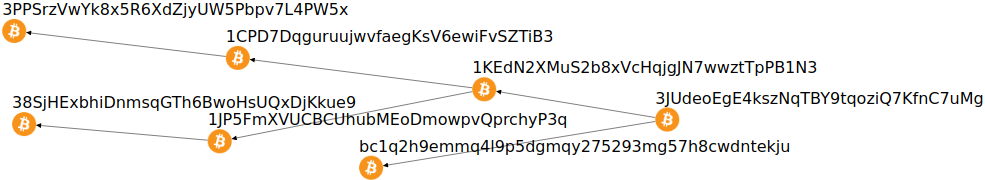
\includegraphics[scale=0.35]{images/exampleWithGraph/complex-tx.png}
\caption{Frammento del grafo delle transazioni relativo alla  transazione descritta nell’Esempio \ref{ex:complexTx}.\label{fig:complexTx}}
\end{figure}

\begin{example} \label{ex:complexTx}
  Considerando il frammento del grafo di address illustrato in Figura \ref{fig:complexTx} dove possiamo osservare la spedizione di bitcoin dall'address \say{3JUd\-eoEg\-E4ksz\-NqTBY\-9tqozi\-Q7Kfn\-C7uMg} verso due nuovi address:

  \begin{itemize}
    \item L'address \say{1KE\-dN2XMu\-S2b8xV\-cHqjgJN\-7wwztTpPB1N3} che rappresenta il destinatario dei bitcoin.
    \item L'address \say{bc1q2\-h9emmq\-4l9p5dgm\-qy27529\-3mg57h8c\-wdnt\-ekju} che rappresenta l'address assegnato all'exchange transaction appartenente al medesimo wallet di origine.
  \end{itemize}
  Dall'address \say{1KE\-dN2XMu\-S2b8xV\-cHqjgJN\-7wwztTpPB1N3} si genera uno spostamento di bitcoin con un ammontare minore del valore rappresentato dal precedente UTXO ricevuto, questo genera due nuove transazioni verso indirizzi distinti, cioè:
  \begin{itemize}
    \item L'address \say{1CPD\-7Dqg\-uruu\-jwvfae\-gKsV6e\-wiFvS\-ZTiB3} che rappresenta il destinatario dei bitcoin.
    \item L'address \say{1JP\-5FmX\-VUCBCUhu\-bMEoDm\-owpvQprch\-yP3q} che rappresenta l'address assegnato all'exchange transaction.
  \end{itemize}

  Dall'address \say{1CPD\-7Dqg\-uruu\-jwvfae\-gKsV6e\-wiFvS\-ZTiB3} avviene uno spostamento di bitcoin verso l'indirizzo \say{3PPS\-rzVwYk8\-x5R6XdZj\-yUW5Pbpv\-7L4P\-W5x} e dall'address \say{1JP\-5FmX\-VUCBCUhu\-bMEoDm\-owpvQprch\-yP3q} avviene uno spostamento di bitcoin verso l'indirizzo \say{38S\-jHExbhi\-DnmsqGT\-h6BwoHs\-UQxDjK\-kue9}, si noti inoltre che gli UTXO vengono \say{consumati} interamente perché non viene generata nessun exchange transaction.

  Questo esempio lascia immaginare che il flusso di bitcoin originato da \say{3JUd\-eoEg\-E4ksz\-NqTBY\-9tqozi\-Q7Kfn\-C7uMg} si sia diretto verso due destinatari diversi: cioè \say{3PPS\-rzVwYk8\-x5R6XdZj\-yUW5Pbpv\-7L4P\-W5x} e \say{38S\-jHExbhi\-DnmsqGT\-h6BwoHs\-UQxDjK\-ku\-e9}, ma questi due address appartengono allo stesso wallet.\\
  Attraverso questa osservazione viene fornita una dimostrazione del problema relativo alla frammentazione degl'address (descritti in dettaglio nella Sezione \ref{sec:grafoDegliAddressProblema}), i quali se utilizzati nel modo giusto possono rappresentare all'interno del grafo un entità distinta.
  Inoltre ad oggi sulla rete bitcoin gli address originati da script sono in rapida crescita, anche perché alcuni software generano solo address derivati da script gestendo internamente le chiavi pubbliche, nascondendo quest'ultime anche al proprietario del wallet.
  Questo rende gli address primitivi catalogabili come address \emph{legacy}.
\end{example}
% ------------------------ End new -------------------------
\section{Grafo delle transazioni} \label{sec:grafoDelleTransazioniProblema}

Il grafo delle transazioni è un grafo diretto i cui nodi rappresentano transazioni e i cui archi denotano il consumo di transazioni da parte di altre transazioni. Come illustrato nel Capitolo \ref{chap:bitcoin}, questo grafo può essere costruito sfruttando i backlink contenuti all’interno delle transazioni di input.

\begin{example}

Consideriamo nuovamente l’Esempio \ref{example:aliceBobFirst}, nel quale Alice vuole trasferire 0.00700767 bitcoin a Bob. Esaminando la nuova  transazione prodotta da Alice e indirizzata a Bob con l’id \say{ddd587d\-54b693\-a9bc9bda\-2218c6f5e17\-979f6ac53755\-c5c1f668f3fa\-728e472d}, possiamo osservare che all’interno della transazione di input era contenuto un id di transazione appartenente ad un precedente UTXO in possesso di Alice (\say{a57c2a4\-27dfa\-591b1243\-343c8413\-c249faac\-3e5df2fe\-4fa1fc93dca\-3d904f3c7}). Conseguentemente, il frammento di grafo corrispondente a questo scambio di bitcoin, mostrato in Figura \ref{fig:graphtxproblem}, contiene due nodi, il primo dei quali corrisponde all'UTXO di Alice, mentre il secondo alla transazione di Alice verso Bob.

\begin{figure}[H]
\centering
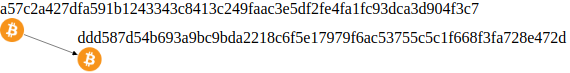
\includegraphics[scale=0.35]{images/exampleWithGraph/aliceBoxTx.png}
\caption{Frammento del grafo delle transazioni relativo alla  transazione tra Alice e Bob descritta nell’Esempio \ref{example:aliceBobFirst}.\label{fig:graphtxproblem}}
\end{figure}

\end{example}

\section{Grafo degli address} \label{sec:grafoDegliAddressProblema}

Il grafo degli address è un grafo diretto i cui nodi sono address e i cui archi rappresentano flussi di bitcoin da un address ad un altro, indotti direttamente o indirettamente da transazioni Bitcoin.

La creazione di questa tipologia di grafi è molto meno intuitiva, poiché, come visto nel Capitolo \ref{chap:bitcoin}, le transazioni non contengono alcun riferimento esplicito a wallet o persone, sfruttando, invece, chiavi private e corrispondenti chiavi pubbliche. Gli address generati attraverso la chiave pubblica sono contenuti all’interno dello script di blocco in modo da rendere la transazione sbloccabile solo dal proprietario della chiave pubblica. \\
Come descritto nella Sezione \ref{sec:bitcoinScriptBitcoin}, gli address possono essere originati anche da uno script tipo P2SH, P2WPKH e P2WSH; ciò rende la creazione del grafo degli address molto insidiosa, perché gli address ricavati dagli script (se utilizzati correttamente) sono univoci e quindi rappresenterebbero un’identità diversa all’interno del grafo, anche se molti di questi potrebbero appartenere in realtà allo stesso wallet.

\begin{example}
Consideriamo nuovamente l’Esempio \ref{example:aliceBobFirst}. In tale esempio  Alice genera una nuova transazione consumando un suo UTXO con un valore maggiore o uguale alla quantità  di bitcoin che desidera trasferire; nell'esempio viene utilizzato un UTXO con un quantitativo maggiore, il che comporta così la generazione di una exchange transaction per riaccreditare la somma eccedente attraverso un nuovo UTXO.

Modellare questo semplice trasferimento può portare a due problematiche.

\begin{itemize}
  \item L’exchange transaction potrebbe contenere un address differente: in questo specifico caso la transazione contiene un address ricavato da uno script Witness (che potrebbe essere ricavato dalla medesima chiave pubblica o da chiavi pubbliche distinte contenute all’interno del wallet).

  \item L'exchange transaction potrebbe contenere uno script P2PKH e quindi un indirizzo primitivo, ma quest’ultimo potrebbe essere differente dall’address di origine. Questo lascerebbe pensare che i bitcoin  siano diretti verso un nuovo proprietario, mentre nella maggior parte dei casi è solo una tecnica per aumentare la privacy utilizzata dagli wallet.
Infatti, molti  wallet comunemente utilizzati contengono un set di chiavi private che permette loro di generare un address diverso ad ogni nuova operazione.
\end{itemize}

\end{example}

La creazione del grafo degli address comporta quindi una serie di problematiche riguardanti gli address, che possono rivelarsi molto significative.

\paragraph*{Indirizzi originati da script}  Il destinatario potrebbe usare indirizzi originati da script (come un address P2SH) rendendo così difficile associare l’appartenenza allo stesso wallet di più address; in alternativa,  l’address potrebbe camuffare uno script P2MS N:M con destinatari distinti. \\
  % ------------------------ Start new -------------------------
  In Figura \ref{fig:alicebobgraphaddress} viene rappresentato il grafo di address coinvolti nell’Esempio \ref{example:aliceBobFirst}, dove l’address \say{33mMAc6nGyENdKMQTr5SrKoEkwNTeZQUx9} rappresenta una particolare tipologia di indirizzo utilizzato da Bob, infatti l'address è ricavato da uno script P2WSH e come illustrato
  nella sezione \ref{sec:p2msbitcoin} l'utilizzo di questo script viene introdotto per ridurre la complessità nella composizione di uno script P2MS; infatti Alice inserisce l’address di Bob all'interno lo script di blocco; Bob per sbloccare questa transizione oltre a fornire la sua firma deve inserire anche lo script di riscatto (illustrato nella sezione \ref{sec:p2msbitcoin}) all’interno lo script di sblocco. \\
  Attraverso questo metodo offerto da Bitcoin Script, Bob può aumentare la sua privacy utilizzando un'indirizzo ricavato da uno script, il quale utilizza due address distinti appartenenti allo stesso wallet.\\
  %------------------------ End new -------------------------
  Gli address che iniziano per \say{bc1q} appartengono al medesimo wallet di Alice; i nodi corrispondenti sono collegati attraverso un arco corrispondente ad una exchange transaction.

\begin{figure}
\centering
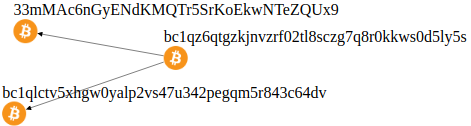
\includegraphics[scale=0.43]{images/exampleWithGraph/exchange-transaction-alice-bob.png}
  \caption{Frammento del grafo di address corrispondente alla transazione illustrata nell’Esempio \ref{example:aliceBobFirst}.\label{fig:alicebobgraphaddress}}
\end{figure}

\paragraph*{Address ricavati da chiavi pubbliche diverse} La generazione delle exchange transaction contiene, nella maggior parte dei casi, un address ricavato da una chiave pubblica diversa, appartenente allo stesso wallet, come illustrato nel seguente esempio.

\begin{example} \label{example:newalicebobaddress}
   Si consideri un nuovo scenario dove Alice spedisce dei bitcoin a Bob ed entrambi i partecipanti utilizzano address primitivi: Alice invia all’indirizzo di Bob 0.00336527 bitcoin, generando una nuova transazione con il seguente id \say{8b22a9\-d19ee58ee1\-b5283632f70\-fbeceaf13\-948dbc3d\-48ea22c02\-1a1d82\-e1f06} verso l’address di Bob \say{1CP\-D7Dqgu\-ruujwvfa\-egKsV6ew\-iFvSZTiB3}.
    Il wallet di Alice utilizza un suo UTXO per effettuare la spedizione di bitcoin con un valore maggiore del necessario, quindi il wallet è costretto a generare una exchange transaction per dividere UTXO. \\
    L’UTXO di Alice con un valore di bitcoin pari a 0.00682055 bitcoin si frammenta in due nuove transazioni:

    \begin{itemize}
      \item La transazione verso Bob del valore di 0.00336527 bitcoin.
      \item L’exchange transaction verso il wallet di Alice del valore di 0.00341851 bitcoin.
    \end{itemize}

La Figura \ref{fig:newalicebobaddress} rappresenta il grafo risultante degli address coinvolti.

\begin{figure}[H]
\centering
    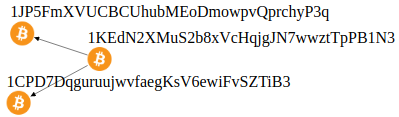
\includegraphics[scale=0.43]{images/exampleWithGraph/example-p2pkh-exchange-transaction.png}
    \caption{Frammento  del grafo degli address coinvolti nella transazione dell’esempio \ref{example:newalicebobaddress}.\label{fig:newalicebobaddress}}
\end{figure}

    In Figura \ref{fig:newalicebobaddress} si possono osservare tre address distinti originati da chiavi pubbliche distinte, dove però i proprietari sono solo Alice e Bob:
    \begin{itemize}
      \item Gli address di Alice sono:
      \begin{enumerate}
      \item \say{1KE\-dN2XMu\-S2b8xVc\-HqjgJN\-7wwztT\-pPB1N3}, che rappresenta l’address di origine;

      \item \say{1JP5F\-mXVUCB\-CUhubME\-oDmowpv\-Qprchy\-P3q} che rappresenta l’address a cui viene indirizzata l’exchange transaction. Entrambi gli address appartengono al wallet di Alice, ma sono originati da chiavi pubbliche diverse.
      \end{enumerate}
      \item L’address di Bob inviato ad Alice per eseguire la spedizione di Bitcoin: \say{1CPD7Dq\-guruujwvf\-aegKsV6ew\-iFvSZTiB3}.
    \end{itemize}
  \end{example}

Nelle prime versioni di Bitcoin, non tutti i wallet contenevano un set di chiavi private e questo comportava la creazione di exchange transaction verso il medesimo address, come mostrato nell'esempio \ref{ex:sameaddr}.

\begin{example}\label{ex:sameaddr}

  Prendiamo in esame la transazione con il seguente id \say{15bf\-8b35c\-9210efe7\-e448\-c5fc6b69b47b3a8\-cac9c148c7cc\-57c65f266\-384d9b8} in cui possiamo osservare la presenza dell’address \say{1EinmJDn\-33yFPGafKu\-Cw2guUqPSMaNKo5v} sia in output che in input.
  La Figura \ref{fig:exchangeaddressrecicle} rappresenta la transazione ricercata attraverso un esploratore blockchain.

\begin{figure}
\centering
  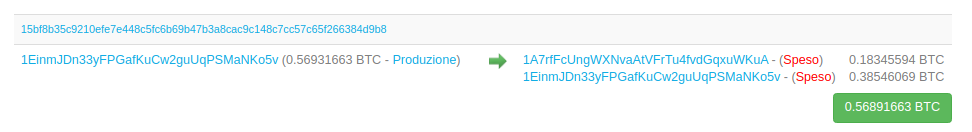
\includegraphics[scale=0.35]{images/exampleWithGraph/exchange-tx-with-same-address.png}
  \caption{Una exchange transaction verso lo stesso indirizzo di origine \cite{blockstream:esplora}.\label{fig:exchangeaddressrecicle}}
\end{figure}

  In questo caso il flusso di bitcoin è chiaro e il corrispondente grafo degli address è mostrato  nella Figura \ref{fig:graphAddresssameaddresschange}.

\begin{figure}[H]
\centering
  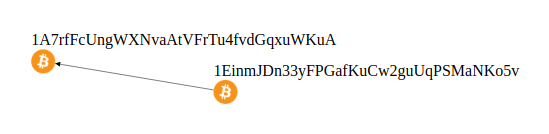
\includegraphics[scale=0.48]{images/exampleWithGraph/exchange-tx-with-same-address-graph.png}
  \caption{Il grafo degli address coinvolti nella transazione con id 15bf8\-b35c9210\-efe7e448c5fc\-6b69b47b3a\-8cac9c14\-8c7cc57c6\-5f26638\-4d9b8.\label{fig:graphAddresssameaddresschange}}
\end{figure}
\end{example}

La costruzione del grafo degli address, oltre ad essere insidiosa per i problemi relativi alla frammentazione degli address, costringe ad accedere alle transazioni di output contenute all’interno delle transazioni, il cui riferimento risiede nelle transazioni di input della nuova transazione, per prelevare l’address di origine.
% --------- For moment I'm comment the figure
%La Figura \ref{fig:processgetorigin} illustra il procedimento per ottenere l’address di origine dell’Esempio \ref{example:aliceBobFirst}.

%{\vspace{15pt}
%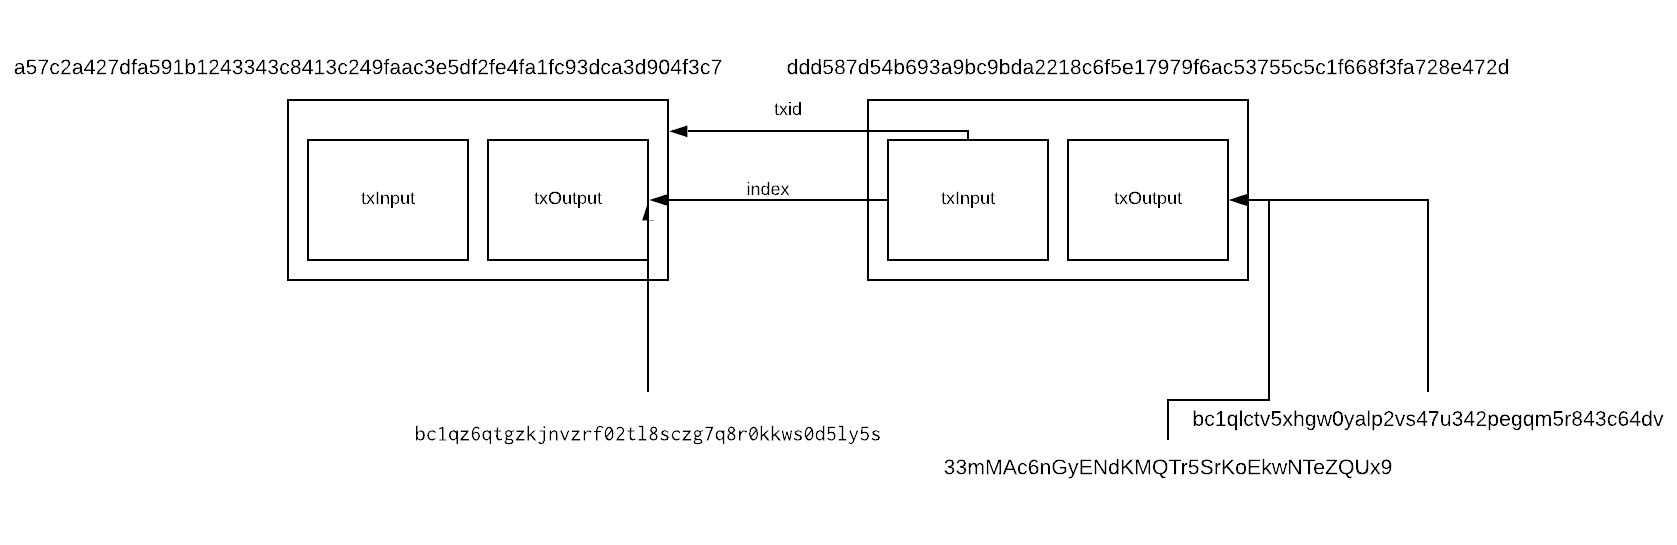
\includegraphics[scale=0.25]{images/howFindTheAddressTo.png}
%\captionof{figure}{Rappresentazione del procedimento per determinare l’address di origine.\label{fig:processgetorigin}}
%\vspace{10pt}
%\par}
